\chapter{Methodology}\label{ch:methodology}

\section{Context and data}

% Where did I take the data from?
% Reddit
% Colleagues and friends

The data was taken from Reddit. I used a technique to motivate users to give me the data. The more data is gather the more money is provided to the charity.

Done during holiodays, no direct concact, only online, so gicing physiucal reqards problematic, steam cards kinda illegal, so this motivation withg  charity seems reasonable. Although, thew research sugguets it may not contribute to increasued attendance in a significant way. Although the times are hard, so it maybe changed.

% Look in the similar papers.

% How did I encourage the people?

\section{Premise}

I utilize the 30 seconds long intervals in order to provide enough High granularity and prevent user Authentication which may happen if intervals were to be too short according to the article. The main purpose of the user interface, that is the dashboard, is to make the users more comfortable with the tool, to enhance trust in it and to encourage them to use it to show them that it makes any sense.

% TODO Mention flow instead probably
\section{Schema of the tool}

User's action triggers changes in the open source files. By the open source files I mean those which are open in the editor. These changes cause text document change events to be emitted. These events are then captured by the internal system. The internal system serves a few purposes. It is responsible for saving the data in the file system, compressing the data and sending it to the cloud storage (Dropbox), as well as controlling the functions of the user interface that is the dashboard.

\begin{figure}[h]
  \centering
  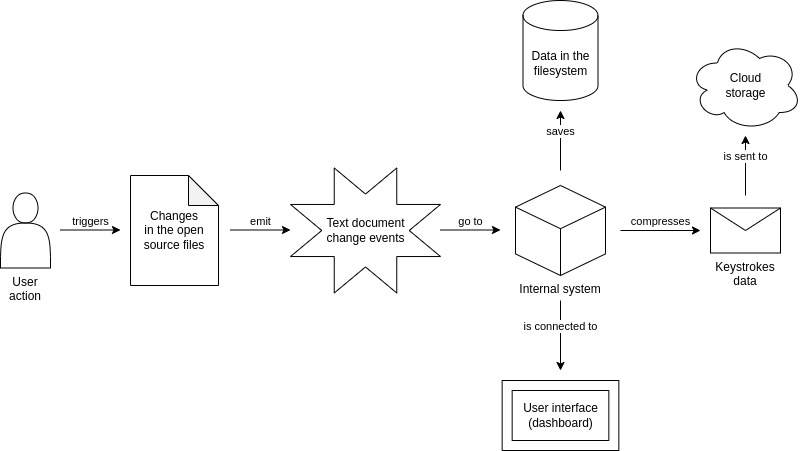
\includegraphics[scale=0.5]{chapters/coding_process_tracker.png}
  \caption{Flow schema of the tool}
\end{figure}

\section{Chosen parts of the tool}

The main component of the internal system are the two buffers filled with the intervals. One of these buffers is the live buffer. The live buffer contains the data gathered lately. It is responsible for creating new intervals from the data that is coming from the user in the real time. The code remembers to save the data in the file system in order to preserve it and not lose it after potential crashes or closing the tool. After saving the data it is possible to remove some intervals from the live buffer in order to be aware of its size and not to allow it to get too big and the memory. The other of the buffers is the static buffer. It is responsible for loading the data from the file system in order for it to be then transferred to the dashboard. The user requests the data from the dashboard.

In order for for the intervals to be visualized they need to be normalized that is made to be of equal lengths. But 0 data you start with the intervals of varying lengths that is of length at most 30 seconds. We need to make them of equivalence and sometimes with that it will equal length being adjustable. Normalization recognizes also that the intervals need to stick to each other however in the Raw data there exist breaks that is there are situations where for some time there is no data start in the file system. So basically we can treat the time spaces that is not covered by the data as intervals with zero keystrokes. Then by interpreting this data such way we can proceed with interpolation let's mention in the figure here. We can imagine that we delete the requested time space into intervals of equal length and then we check if they intersect with the intervals from the real data. The amount of keystrokes that the new interval receives is proportional to the relative size of the intersection to the length of the whole row interval. So it's about you looking at the example from the figure if the intersection constitutes 30\% of the row interval then then we take into account 30\% of keystrokes from this row interval to the new interval of equivalent. The total number of keystrokes associated with this new interval is calculated by summing all of the keystrokes associated with all the intersections from the different row intervals which we can see in the future Maybe we'll delete it later I think.

The user interface constitutes the dashboard that a user can use to view various statistics across different time periods. it is possible through switching modes. The first mode is called the live view.  In this view a user is able to view the latest data. She can also adjust the  time gauge to explore the data in the different time periods (rather in the different lengths from now). The user is provided also with the Calendar view. It is utilized to explore the data from previous days. After selecting today the user can also adjust the time period by using the aforementioned gauges. The parameters of the plot are adjusted automatically in order for the blood to be visible to the user. That means not too convoluted, not too cluttered. The dashboard is connected with the live and static buffers and depending on the View the data is loaded from the light buffer or from the static buffer (that is indirectly from the file system).

\begin{figure}[htbp]
  \centering
  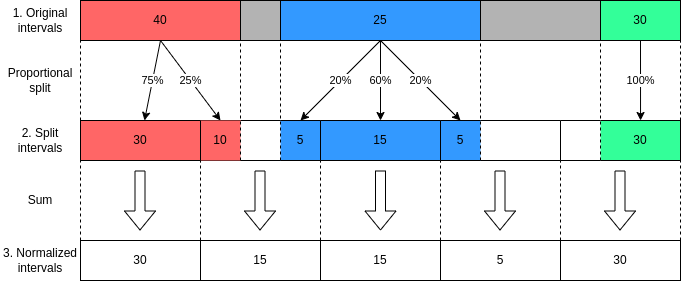
\includegraphics[scale=0.5]{chapters/normalization.png}
  \caption{An intervals normalization example}
\end{figure}

\begin{figure}[htbp]
  \centering
  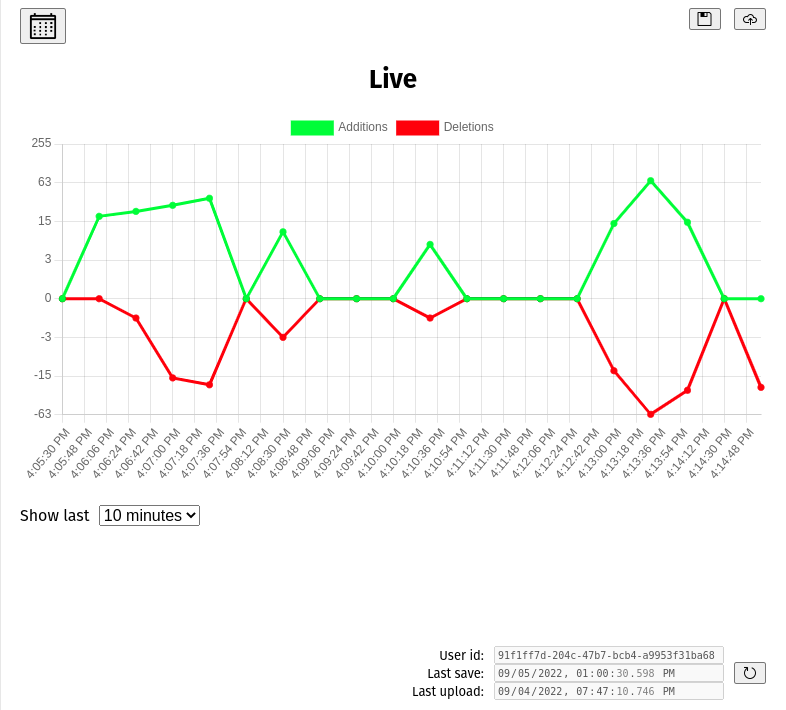
\includegraphics[scale=0.5]{chapters/live-view.png}
  \caption{Live view of the dashboard}
\end{figure}

\begin{figure}[htbp]
  \centering
  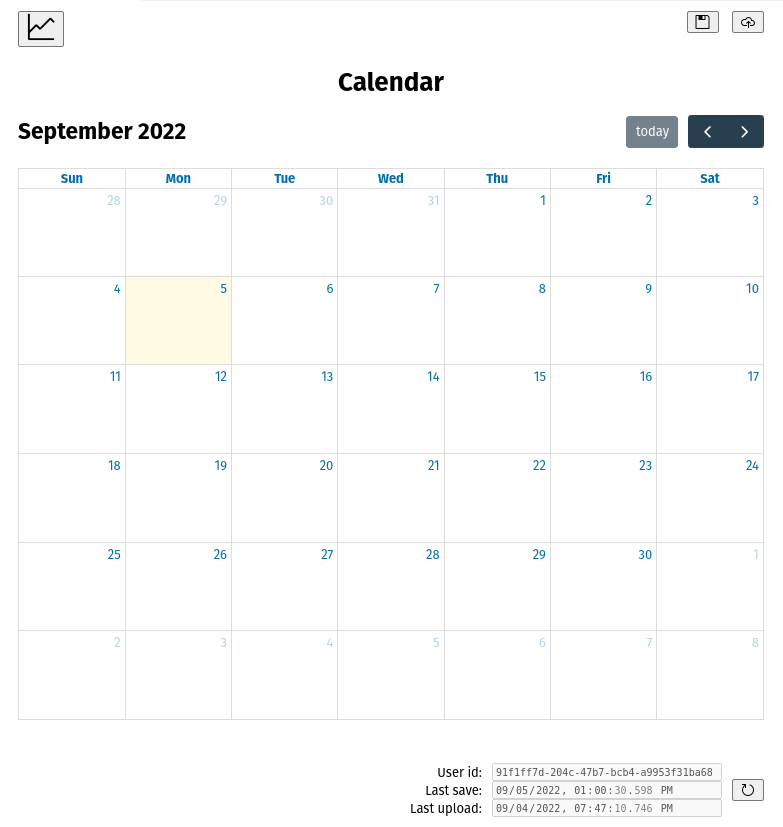
\includegraphics[scale=0.5]{chapters/calendar-view.png}
  \caption{Calendar view of the dashboard}
\end{figure}

\begin{figure}[htbp]
  \centering
  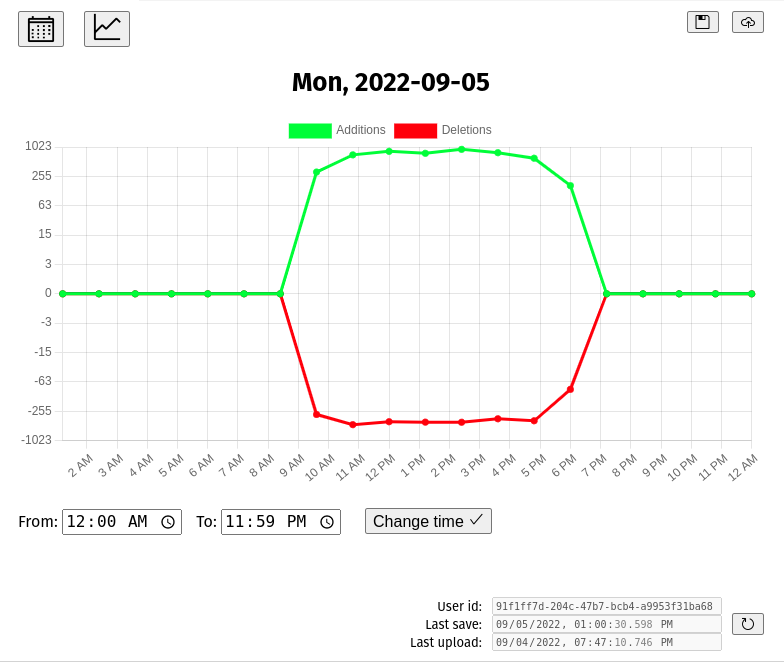
\includegraphics[scale=0.5]{chapters/day-view.png}
  \caption{Day view of the dashboard}
\end{figure}

% TODO file name (not underscore)
\begin{figure}[htbp]
  \centering
  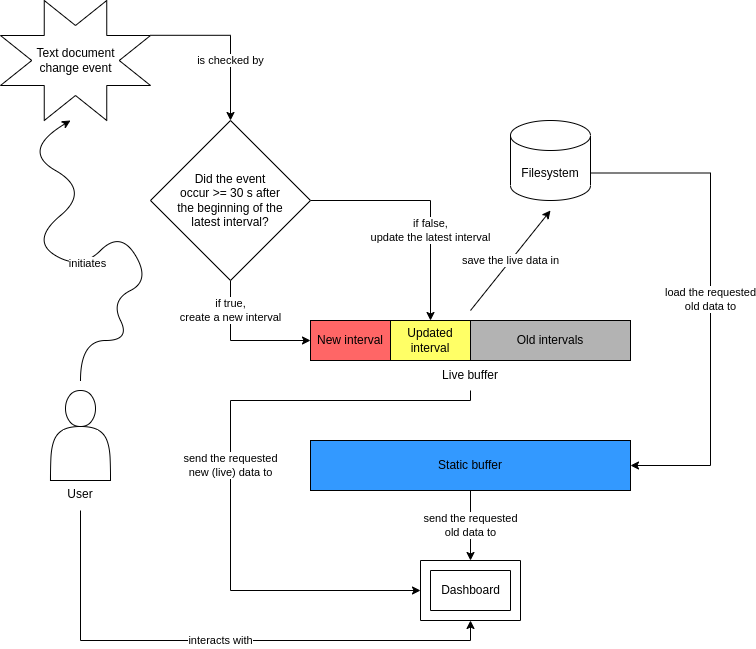
\includegraphics[scale=0.5]{chapters/internal_system.png}
  \caption{Internal system}
\end{figure}

\section{Methods of data analysis}

In the species I will perform a few analytical tests on The Gather the data. This test will include measuring the average length of breaks, their frequency. I will measure the correlations between additions and deletions I will analyze the additions to deletions ratio. I will try as well too observe the existence of morning and evening chronotypes. I will do that bye searching for time periods of particularly increased or decreased activity. I will observe that frequency of extreme points in the plots. This way I can make hypothesis about the actual real actions of programmers because for instance in the Version Control systems merging code may result in high numbers of auditions or deletions. I mean that such suspicious pics of activity May provide evidence to particular actions. Of course I will examine the data also with the with respect to the different programming languages. This way I might find some statistical features that are specific to a particular language.
